\documentclass{standalone}

\renewcommand{\familydefault}{\sfdefault}
\usepackage{amsmath}
\usepackage{tikz}
\usetikzlibrary{arrows.meta, positioning, calc, }

\begin{document}

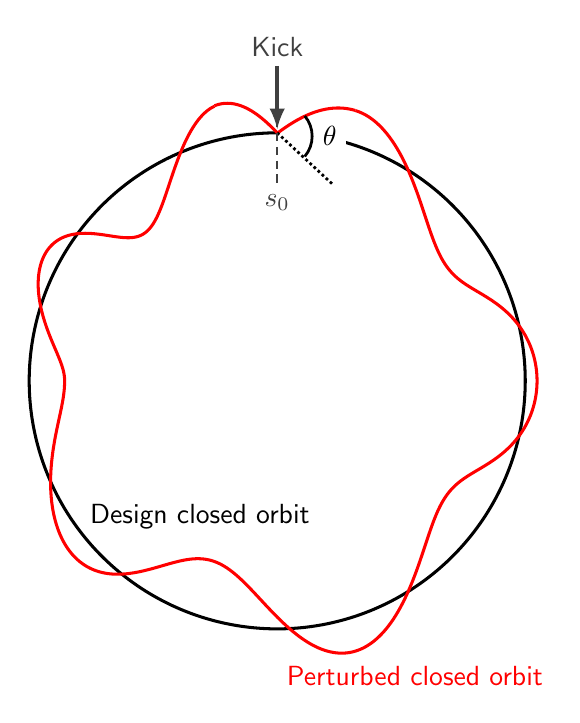
\begin{tikzpicture}[>=latex]
    % a orbita fechada ideal/desing
    % \draw[black, thick] (0, 0) circle (3.1);
    \draw[domain=10:360, variable=\t, samples=500, black, line width=1.1pt, scale=3.15] plot (
    {sin(\t)}, 
    {cos(\t)});

    \pgfmathsetmacro{\rangem}{270}
    
    
    \draw[domain=17.5:\rangem, variable=\t, samples=500, red, scale=3, line width=1.1pt] plot (
    {(1 + 0.1*sin(5*\t))*sin(\t)}, 
    {(1 + 0.2*sin(5*\t)) * cos(\t)});

    \draw[domain=\rangem:360-14, variable=\t, samples=500, red, scale=3, line width=1.1pt] plot (
    {(1 - 0.1*sin(7*\t)) * sin(\t)}, 
    {(1 - 0.2*sin(7*\t)) * cos(\t)}
    );

    \draw[domain=0:17.5, variable=\t, samples=500, red, scale=3, line width=1.1pt] plot (
    {(1 + 0.1*sin(5*\t)) * sin(\t)}, 
    {(1 + 0.15*sin(5*\t)) * cos(\t) + 0.048});

    \draw[domain=360-14:360, variable=\t, samples=500, red, scale=3, line width=1.1pt] plot (
    {(1 - 0.1*sin(7*\t)) * sin(\t)}, 
    {(1 - 0.15*sin(7*\t)) * cos(\t) + 0.05}
    );

    % \draw[->] (-4, 0) -- (4, 0) node[right] {$x$};
    % \draw[->] (0, -4) -- (0, 4) node[right] {$y$};

    \draw[densely dotted, line width=1pt] (0, 3.15) -- (0.7, 2.50); 

    \draw[line width=1pt] (0.35, 2.85) arc (-40:40:0.4) node[midway, right, fill=white] {$\theta$}; 

    \draw[densely dashed, darkgray, line width=0.8pt] (0, 3.5) -- (0, 2.5) node[below] {$s_0$};
    \node[darkgray, above] at (0, 4) {Kick};
    \draw[darkgray, ->, line width=1.5pt] (0, 4) -- (0, 3.2);

    \node[black, above right] at (-2.5, -2) {Design closed orbit};
    \node[red, below right] at (0, -3.5) {Perturbed closed orbit};

\end{tikzpicture}


\end{document}
